\documentclass[a4paper, dvipdfmx]{ujarticle}
\usepackage[T1]{fontenc}
\usepackage{graphicx}

%\input{macro}

\topmargin -28mm
\oddsidemargin -15mm
\evensidemargin -15mm
\textwidth 185mm
\textheight 275mm
\columnsep 6mm

\def\toujitu{令和9年2月12日}

% \Eps{filename}{caption}{label}{scale}
%\newcommand{\Eps}[4]{ \begin{figure}[hbtp] \begin{center} \psbox[scale=#4]{#1} \end{center} \vspace{-8mm} \caption{#2} \label{#3} \end{figure} }

\makeatletter
\def\section{\@startsection{section}{2}{\z@}{.8ex plus .8ex minus 
 .2ex}{.05ex plus .07ex}{\large\bf}}
\makeatother
\makeatletter
\def\subsection{\@startsection{subsection}{2}{\z@}{.8ex plus .8ex minus 
 .2ex}{.05ex plus .07ex}{\bf}}
\makeatother


\pagestyle{empty}

\begin{document}

\baselineskip 4.75mm
%行間の指定をここで行う

\twocolumn
[
\footnotesize 
\begin{center}
{大阪大学大学院情報科学研究科 マルチメディア工学専攻 博士前期課程修士学位論文発表会資料
\hfill \toujitu}\\
\medskip
{\large
{\bf マルチメディア工学専攻における修士学位論文発表会資料サンプル}\\
}
\medskip
{\large
高橋 拓豊 (先進高性能計算基盤システム講座)
}
\end{center}
]

\section{はじめに}
高性能計算 (HPC) アプリケーションにおいて，プログラムの高速化は非常に重要な課題であり，さまざまな状況で要求されている．
プログラムの実行時間は実行環境や入力データに応じて設定すべきチューニング対象の性能パラメータに大きく依存する．
性能パラメータの最適な組合せはアプリケーションや実行環境によって異なるため，その最適化を人手で行うには多大な労力を要する．
そのため，実行時間の性能パラメータを自動的に探索する自動チューニングが活発に研究されている．

自動チューニングの代表的なアプローチとして，機械学習に基づく性能モデルを用いた手法が広く研究されている．
これらの手法では，対象アプリケーションの実行時間を評価しながら，評価済みの性能パラメータの設定と実行時間の関係から性能モデルを構築し，多数の候補の中から有望な設定を選択することで，少ない評価回数で高性能な設定を探索する．
しかし，性能パラメータと実行時間の関係のみを学習する性能モデルでは，プログラム実行時のハードウェア内部挙動を扱えていない．
性能パラメータの違いによって生じる実行時間の差には，キャッシュミスや分岐予測ミスなどのハードウェア内部挙動が影響する．

本研究では，ハードウェア内部挙動として性能カウンタを用いることで得られるキャッシュミス率などの性能カウンタ値を活用することで，自動チューニングにおける探索時間の評価回数の削減を目指す．


\section{提案}
既存の性能モデルに基づくオートチューニングでは，

\begin{figure}[t]
    \centering
    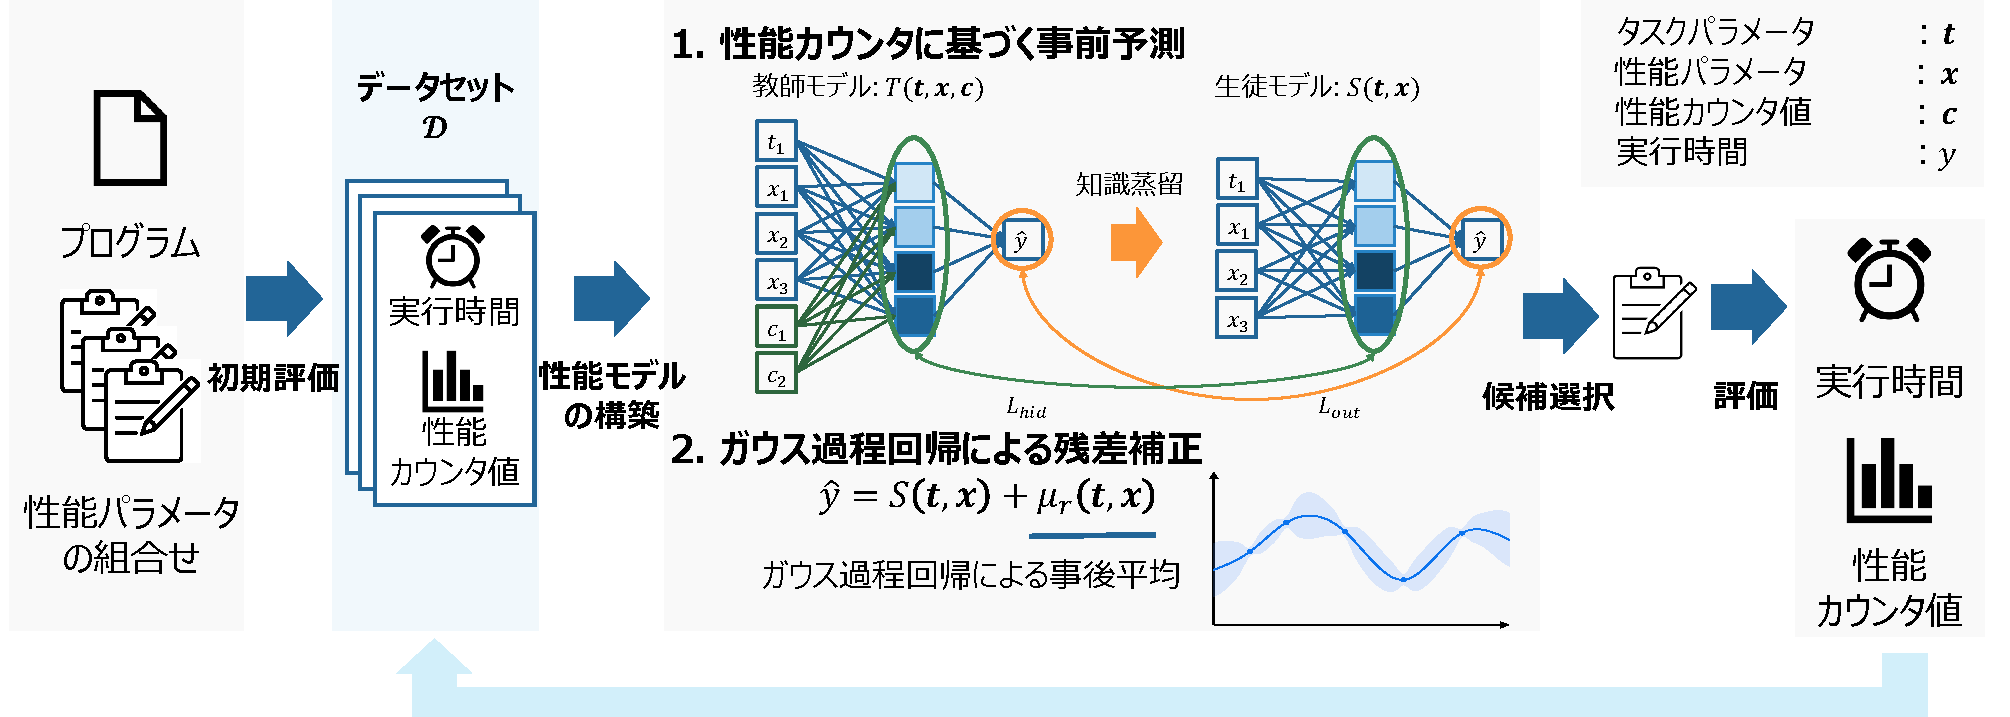
\includegraphics[width=\columnwidth]{prop_ja.pdf}
    \caption{提案手法の概要図}
    \label{fig:prop}
\end{figure}


\section{評価}

\section{まとめ}

\end{document}
















